% Options for packages loaded elsewhere
\PassOptionsToPackage{unicode}{hyperref}
\PassOptionsToPackage{hyphens}{url}
%
\documentclass[
]{article}
\usepackage{amsmath,amssymb}
\usepackage{lmodern}
\usepackage{iftex}
\ifPDFTeX
  \usepackage[T1]{fontenc}
  \usepackage[utf8]{inputenc}
  \usepackage{textcomp} % provide euro and other symbols
\else % if luatex or xetex
  \usepackage{unicode-math}
  \defaultfontfeatures{Scale=MatchLowercase}
  \defaultfontfeatures[\rmfamily]{Ligatures=TeX,Scale=1}
\fi
% Use upquote if available, for straight quotes in verbatim environments
\IfFileExists{upquote.sty}{\usepackage{upquote}}{}
\IfFileExists{microtype.sty}{% use microtype if available
  \usepackage[]{microtype}
  \UseMicrotypeSet[protrusion]{basicmath} % disable protrusion for tt fonts
}{}
\makeatletter
\@ifundefined{KOMAClassName}{% if non-KOMA class
  \IfFileExists{parskip.sty}{%
    \usepackage{parskip}
  }{% else
    \setlength{\parindent}{0pt}
    \setlength{\parskip}{6pt plus 2pt minus 1pt}}
}{% if KOMA class
  \KOMAoptions{parskip=half}}
\makeatother
\usepackage{xcolor}
\usepackage[margin=1in]{geometry}
\usepackage{longtable,booktabs,array}
\usepackage{calc} % for calculating minipage widths
% Correct order of tables after \paragraph or \subparagraph
\usepackage{etoolbox}
\makeatletter
\patchcmd\longtable{\par}{\if@noskipsec\mbox{}\fi\par}{}{}
\makeatother
% Allow footnotes in longtable head/foot
\IfFileExists{footnotehyper.sty}{\usepackage{footnotehyper}}{\usepackage{footnote}}
\makesavenoteenv{longtable}
\usepackage{graphicx}
\makeatletter
\def\maxwidth{\ifdim\Gin@nat@width>\linewidth\linewidth\else\Gin@nat@width\fi}
\def\maxheight{\ifdim\Gin@nat@height>\textheight\textheight\else\Gin@nat@height\fi}
\makeatother
% Scale images if necessary, so that they will not overflow the page
% margins by default, and it is still possible to overwrite the defaults
% using explicit options in \includegraphics[width, height, ...]{}
\setkeys{Gin}{width=\maxwidth,height=\maxheight,keepaspectratio}
% Set default figure placement to htbp
\makeatletter
\def\fps@figure{htbp}
\makeatother
\setlength{\emergencystretch}{3em} % prevent overfull lines
\providecommand{\tightlist}{%
  \setlength{\itemsep}{0pt}\setlength{\parskip}{0pt}}
\setcounter{secnumdepth}{5}
\ifLuaTeX
  \usepackage{selnolig}  % disable illegal ligatures
\fi
\IfFileExists{bookmark.sty}{\usepackage{bookmark}}{\usepackage{hyperref}}
\IfFileExists{xurl.sty}{\usepackage{xurl}}{} % add URL line breaks if available
\urlstyle{same} % disable monospaced font for URLs
\hypersetup{
  pdftitle={Using mechanistic models to assess temporary closure management strategies of octopus fisheries},
  pdfauthor={Sophie Wulfing, Easton White, Ahilya Sudarshan Kadba},
  hidelinks,
  pdfcreator={LaTeX via pandoc}}

\title{Using mechanistic models to assess temporary closure management strategies of octopus fisheries}
\author{Sophie Wulfing, Easton White, Ahilya Sudarshan Kadba}
\date{2022-09-08}

\begin{document}
\maketitle

\hypertarget{to-do}{%
\subsection{To do:}\label{to-do}}

Look at paper printour of lifespan.
Insert Ahilya Info.
Which R packages do i Cite.
APPENDIX!
MAKE FIG CAPS FOR EVERYTHING AND EDIT FIGS.
Sensitivity.
Want feedback on sensitivity and elasticity paragraphs, Ahilya's. Formatting pointers.

\hypertarget{introduction}{%
\section{INTRODUCTION}\label{introduction}}

AHILYA PARAGRAPH. REVIEW. Ecological modeling is the employment of mathematics in studying intraspecies and interspecies relationships in addition to predicting future population dynamics when the same species are subject to novel environments or management. This technique plays a critical role in making informed conservation decisions. INTRO MECHANIST AND WHY WE USE Mechanistic models have delivered some promising results to researchers modeling data-deficient species. In 2017, Smallegange et al.~used a mechanistic model to study the relationship between expected feeding level and growth, lifetime reproductive success and generation time for the species \emph{Manta alfredi} (commonly known as reef manta ray). Klok et al.~in 2007 combined the dynamic energy approach with a matrix model to study the effects of environmental toxin, copper, on growth and reproduction of earthworm, Dendrobaena octaedra. Mechanistic models differ from statistical ones in the sense that they use characters of individuals to describe how changes in the environment influence changes in individuals in terms of these characteristics. As a result, they are not reliant on empirical data and extraordinarily applicable to data-deficient species. Furthermore, since mechanistic modeling does not involve following individuals from birth to death to determine parameters, it is extremely beneficial for studying organisms whose life history cannot be tracked individually (Smallegange et al., 2017). One type of mechanistic model are matrix population models. These specialized matrices are used for ``structured populations'' -- populations in which individuals can be categorized based on age, stage, weight or length. They use demographic rates to create a projection matrix -- a square matrix where the number of rows and columns are equivalent to the number of life stages. Transformations of these matrices can be used to predict future population dynamics.

The ocean environments off the southwest coast of Madagascar are home to a wide variety of marine life, as sand beds, seagrass beds and coral reefs are all prominent biomes in the area. Increased urbanization in the region has led to higher fishing pressure which has in turn led to a decline in fish catch and biomass (Laroche et al., 1997). In fact, Madagascar has been calculated to be among the top countries for potential successful preservation based on the potential economic benefits and success of harvest regulation (MacNeil et al., 2020), especially in the western region of the country (Laroche et al., 1997). 32 million fishers make their livelihood in small-scale fisheries, a subsector in which 90 to 95\% of fish is distributed for local consumption. These marine products are a vital source of nutrition for these communities (World Bank, 2012). In the early 2000's, however, Madagascar began to move from local, subsistence fishing to selling and exporting catch to export markets (Humber et al., 2006), and there is evidence that up to 75\% of all fish caught is now sold to outside entities for export (Baker-Médard, 2017).

REREAD:
Marine Protected Areas (MPAs) are regions in the ocean identified as being biologically important and fishing protections are therefore enforced. The type and level of fishing protection can vary depending on the class and goals of the MPA (Grorud-Colvert et al., 2021). Before their establishment in Madagascar, governmental bodies had bans on certain types of fishing gear, implemented seasonal fishing regulations, and criminalized the harvest of endangered species. However, these strategies proved ineffective in execution and in their conservation goals (Humber et al., 2006). Both the government and nongovernmental organizations have since pledged to drastically increase the number of regions dedicated as MPAs through temporary fishing closures (Baker-Médard, 2017; Cinner et al., 2009; Oliver et al., 2015). These temporary restrictions can affect different species differently, and commercially valuable species may not be the ones that respond positively to the reduced fishing pressure (Gilchrist et al., 2020; Grorud-Colvert et al., 2021). On the other hand, the economic benefits after reopening fishing grounds have been seen to outweigh these costs (Oliver et al., 2015; Humber et al., 2006), indicating that they are a useful strategy, but must be implemented with consideration for how the different fish populations and human communities will be affected.

Since 2003, when this resource first began to globalize, cephalopods have become one of the largest classes of exports (Humber et al., 2006; Aina 2009, Barnes-Mauthe et al.~2013). This has since added significant fishing pressure to Madagascar's cephalopod populations and yield from this fishery has decreased in the southwest Andavadoaka region (Humber et al., 2006). Cephalopods are a vital part of many ocean ecosystems and, compared to other fisheries, have a unique life history that can lead to distinct and variable population dynamics. Cephalopods act as both predators and prey in an ecosystem (Rodhouse \& Nigmatullin, 1996; Santos et al., 2001; Vase et al., 2021), situating them in a key role in food webs. They also provide rich nutrition and bioactive compounds to the oceanic microbial community (Catalán et al., 2006; Fitahia et al., 2018; Ibáñez et al., 2019; Van Nieuwenhove et al., 2019). Further, their abundance varies drastically with a wide range of ocean conditions including sea surface and bottom temperature, salinity, currents, and sediment type (Catalán et al., 2006; Ibáñez et al., 2019; Van Nieuwenhove et al., 2019). Compared to other exploited marine organisms, cephalopods have a short lifespan coupled with a fast reproduction rate and high fecundity. This explains their population's ability to quickly bounce back when short term MPAs are introduced into their habitat (Benbow et al., 2014; Humber et al., 2006; Katsanevakis \& Verriopoulos, 2006). However, once fishing resumes, populations suddenly and rapidly decline although in some examples, this could be attributed to heavy fishing pressure in the area right after reopening (Humber et al., 2006). Cephalopods are therefore extremely sensitive to both protection and harvest levels.

\emph{Octopus cyanea}, or blue octopus, is the most abundant cephalopod species in this region and is caught in about 95\% of local landings (Humber et al., 2006; Oliver et al., 2015). Like other cephalopod species, very little is known about their life history including natural death rate, REVIEW AHILYA'S NOTES AND PUT IN HERE. Further, age is difficult to determine from size alone as they have variable growth rates upto maturity (Raberinary and Benbow 2012, Herwig et al., 2012, Heukelem and Fred 1976, Wells and Wells 1970). To protect this species, size limits have been imposed on blue octopus catch in Madagascar, but these regulations are difficult in practice, as blue octopus typically die before size can be assessed (Humber et al., 2006). Therefore, temporary closures have been shown to be a more effective method of blue octopus conservation (Benbow 2014).

Population matrix models are a commonly used mechanistic model to predict future population dynamics by splitting the life history of the study organism up into a Leslie Matrix (Leslie, 1945) where a population is split up into groups of ages, and a transformation matrix is applied to predict what the population makeup will be in future years. However, these models require extremely in-depth data collection to inform each entry of the model, such as yearly survival rate based on age. This is not a reality for many organisms where these kind of data cannot be collected due to the difficulty in monitoring some species in yearly increments (Crouse et al., 1987) and for organisms that have long larval stages, where calculating survival probabilities for this time is nearly impossible (Gharouni et al., 2015). As these obstacles apply to our study species, where there is no existing data on the population of octopus in each age group, we will instead use a stage-based population matrix, otherwise known as a Lefkovitch matrix (Caswell, 2001). Here, the life history of the study organism is grouped by stages, where each unit of the matrix represents a distinct period of the organism's life where it is subject to different environments, pressures, or physical attributes that would alter the survival and reproductive output at that phase, but the amount of time between each stage is now variable. This would simply create different inputs for the probability of remaining in the same stage, and the growth and fecundity inputs can be based on available data. Therefore, the model employed by this project will depend on the life history of each cephalopod species and what data we find available to inform the inputs of the matrix.

In this paper, we have 4 goals: 1) we will fit a Levkovitch matrix to the limited available data on \emph{Octopus cyanea} populations in southwestern Madagascar, 2) determine what conservation actions need to be taken, 3) as well as create a theoretical estimation of the species' life history traits in different stages of its development and 4) we can hopefully determine the frequency and length in which these temporary closures should take place to maximize population health of both the octopus and the local community.

\hypertarget{methods}{%
\section{METHODS}\label{methods}}

CITE R PACKAGES

IDK I DON'T KNOW WHERE YOUR LIFE HISTORY GRAPH FIGS WENT BUT PROBS PUT THAT IN

Data was collected by Raberinary and Benbow (2012) from landings ranging from the villages of Ampasilava in the south to Andragnombala in the north which spans about 30 kilometers of coastline. They collected landing data from February 2005 to February 2006 through daily surveying fishers as they landed onshore within a two hour window. They collected octopus weight, weight and length of gonads, sex, and a visual assessment of maturity class. A subsample of octopus were also collected for octopus length, and laboratory assessment of gonads for a confirmation of maturity class. They collected a total of 3253 octopuses, and for the purposes of this study, we will be modeling from the 1578 females collected. Despite there being no standardization for catch effort being available for this dataset, no other maturity stage study has been conducted on this population of \emph{O. cyanea} and is therefore the best available data to fit a Lefkovitch matrix.

In order to parameterize this model, we used Wood's Quadratic Programming Method outlined in Caswell 2001. Other methods required longer time series than were available to us, were extremely sensitive to noise in the data, or simply resulted in matrices that had no biological interpretation (Caswell 2001). Figure \ref{tab:WriteMtxRounded} WHY WONT THIS WORK?!?! shows a preliminary stage-based matrix model based on Raberinary and Benbow (2012) data. Model accuracy was assessed by comparing life history values inferred from the matrix with existing literature on \emph{O. cyanea} life history (CREATE AND INSERT AHILYA TABLE). As all of our values calculated from the matrix fell within the known attributes of this species, we were confident that this model gave an accurate mechanistic description for this population's underlying dynamics.

Eigenvalues (\(\lambda\)) were then calculated from the matrix, which indicate population growth rate (r) as \(\lambda\) = \(e^r\). Further, future populations can be predicted by multiplying a population vector to incrementally higher powers of our matrix where the power of the matrix corresponds to the time length of the projection.

We performed sensitivity analysis on the population matrix and eigenvalues (RPACKAGE CITE?). The result of this analysis indicates how much the dominant eigenvalue will change as a result of perturbations in each parameter of the matrix (Demetrius 1969). Further, as all of the parameters are scaled to a value between 0 and 1 except \(F_4\), a unit change in these parameters will have a greater proportional effect on the eigenvalue than \(F_4\). To address this, we also conducted elasticity analysis. Similar to sensitivity analysis, elasticity indicates how heavily the growth rate will respond to a proportional change in each parameter in the matrix (de Kroon et al.~1986). This will allow us to identify the groups within this octopus population whose protection will most benefit population growth, essentially creating focus points of conservation. Other life history traits that can be calculated from this matrix are stable stage distribution, reproductive value of each stage, average lifespan, and per-stage survivability.

In order to determine optimal conservation strategies, we altered the survivability of \emph{O. cyanea} by different rates from 0-10\% survival increase of the species. Then, we simulated different closure scenarios for each survival increase, increasing the number of months between closures. We then took the weighted average of the growth rates of the closed and open fishing scenarios for the hypothetical population and analyzed if this resulted in a stable population (i.e if the resulting rate of increase was positive). Pareto (CITE???) analysis was then conducted on these different scenarios in order to analyze all combinations of conservation strategies that result in stable \emph{O. cyanea} populations.

\[\begin{bmatrix}
P1 = 0.63&0&0&F4 = 26.7 \\
G1 = 0.275&P2 = 0.322&0&0 \\
0&G2 = 0.13&P3 = 0.393&0 \\
0&0&G3 = 0.093&P4 = 0.331 \\
\end{bmatrix}\]

\hypertarget{results}{%
\section{RESULTS}\label{results}}

FIX BOOKDOWN
SEE NOTES IN GOOGLE DOC FOR EDITS
The resulting eigenvalue of our matrix was 0.982, indicating a population decline of 1.8\% per month of -0.0184 (Figure \ref{fig:projection}) MAKE FIG CAP. Sensitivity analysis (Figure \ref{sensitivity}) MAKE FIG CAP showed that within each stage, the growth parameters (\(G_1\) - \(G_3\)) had the largest effect on the eigenvalue compared to the parameters indicating staying within a stage (\(P_1\)-\(P_4\)). However, as all the parameters must necessarily be between 0 and 1 with the exception of the \(F_4\) parameter, elasticity analysis provides an interpretation that weights all stages equally. The result of this analysis shows that percent changes in the fecundity metric can be as beneficial to the overall population growth as changes in the G parameters (Figure \ref{fig:elasticity}). Further, this analysis indicates that of all the stages, stage 1 has the most overall influence on the overall population growth. The stable stage distribution (Table \ref(tab:lifetable)) MAKE THIS shows that 65\% of the makeup of this population is immature individuals, while actively breeding individuals (fully mature) only make up less than 1\% of the naturally occurring population. However, the reproductive output per stage (Table \ref(tab:lifetable)) shows that on average, an individual in this fully mature population is expected to have 41 times the number of offspring as those in stage 1.

Our analysis of different closure scenarios \ref{fig:closures}) indicates closures less frequent than once every five months will be ineffective in ensuring a stable population. Further, as our baseline growth rate was close to stable (-0.0184), it took a maximum of a 10\% increase in the survivability of the population to ensure a sustainable population. Our pareto analysis (Figure 6) provides all the possible combinations of increased survival rates and frequency of closures that will result in a stable population. Suggested changes in overall survivability range from 2-10\%, and the ranges of frequencies of closures span from permanent closure (every month) to once every five months.

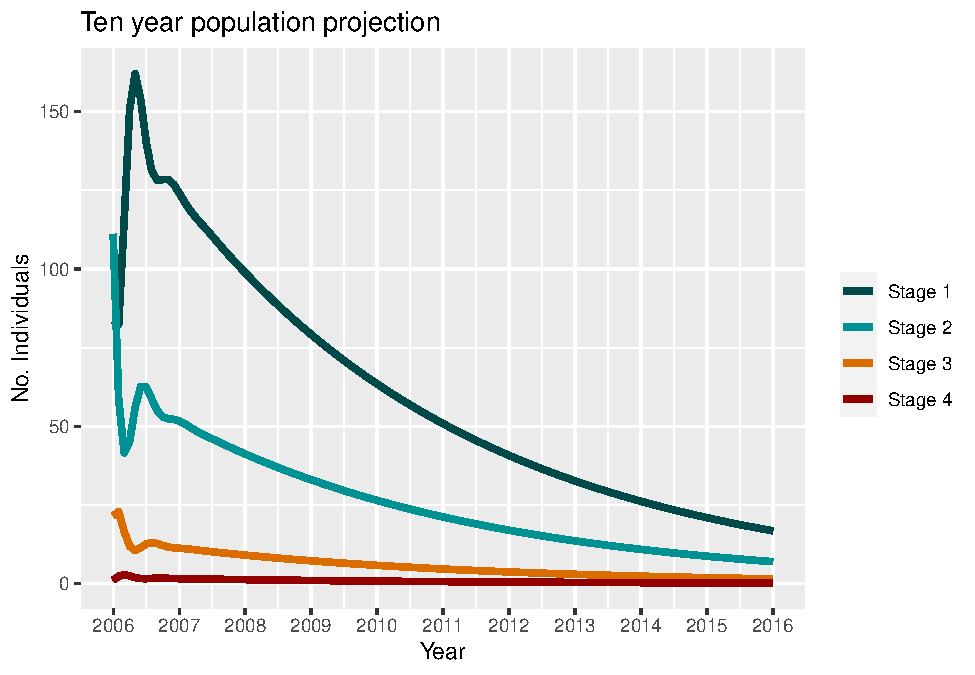
\includegraphics{Wulfing_CH1_Draft1_files/figure-latex/projection-1.pdf}

\begin{figure}
\centering
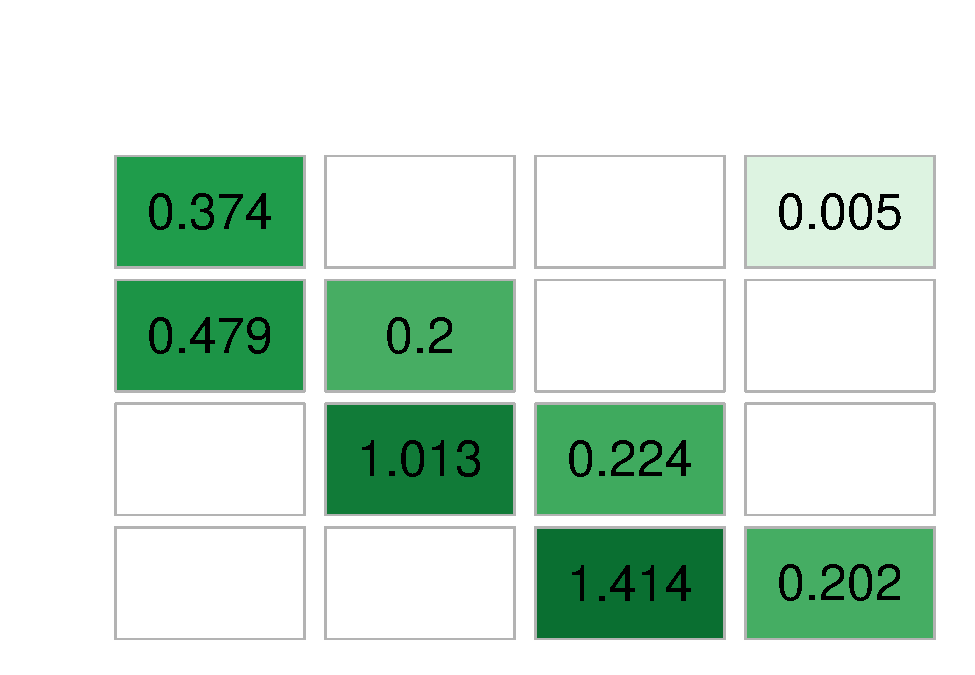
\includegraphics{Wulfing_CH1_Draft1_files/figure-latex/sensitivity-1.pdf}
\caption{\label{fig:sensitivity}Sensitivity analysis \label{sensitivity}}
\end{figure}

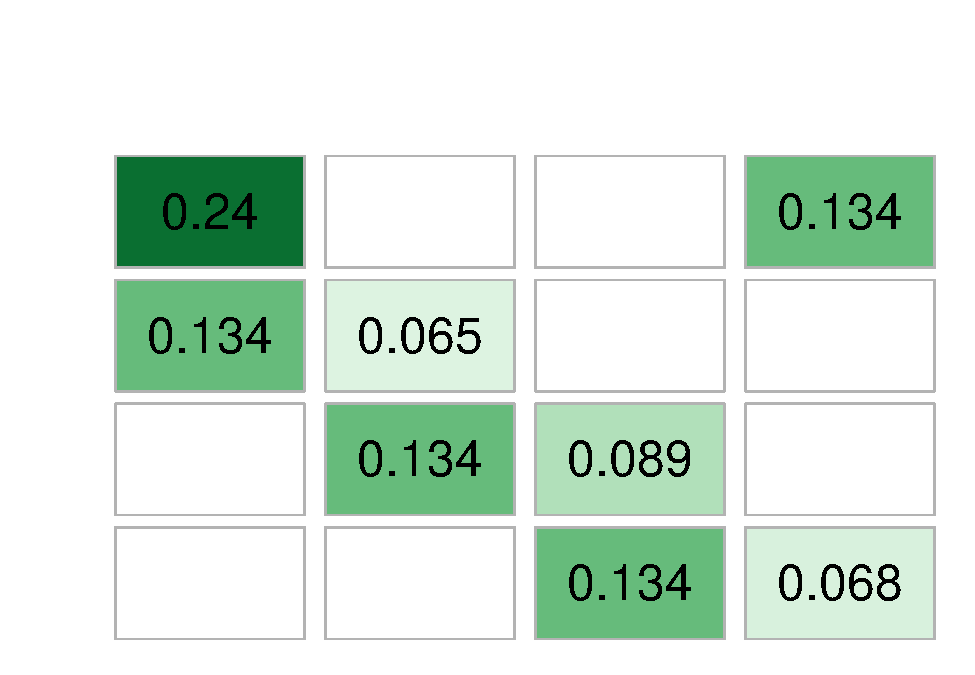
\includegraphics{Wulfing_CH1_Draft1_files/figure-latex/elasticity-1.pdf}

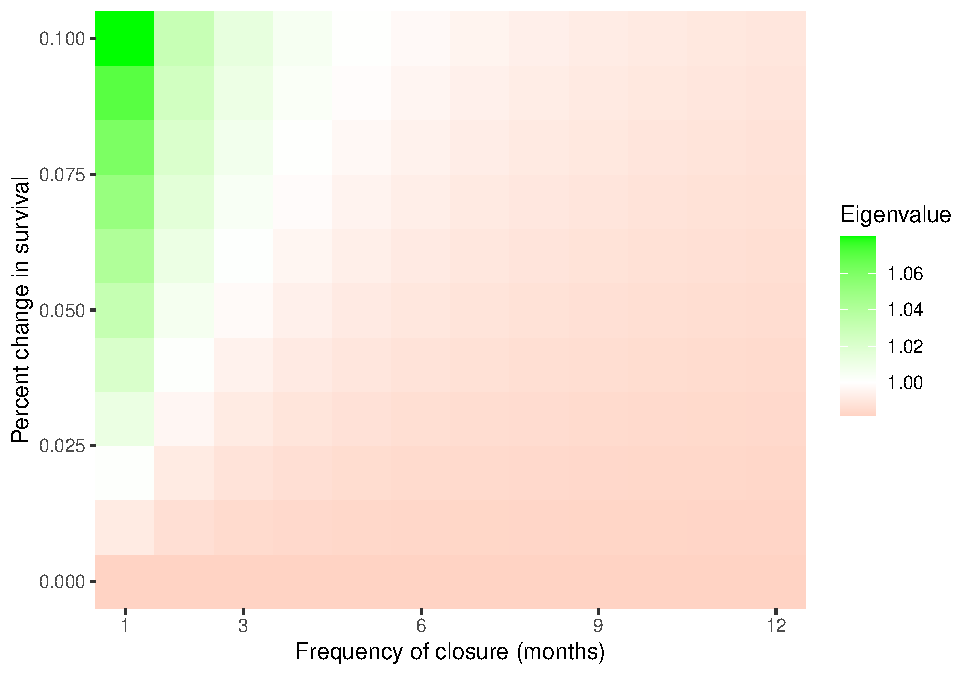
\includegraphics{Wulfing_CH1_Draft1_files/figure-latex/closures-1.pdf}

\hypertarget{discussion}{%
\section{DISCUSSION}\label{discussion}}

MAKE THIS PARAGRAPH LONGER SOMEHOW INCORPORATE LIT?
Our calculated growth rate of -0.0184 and resulting population projection further supports previous reports of declined catch (Humber 2006, Benbow 2014) and indicate an assessment of possible action toward more sustainable practices. Decline in population presents an economical issue for individual fishers as their catch will become less lucrative and a recovery of this population will also result in economic gains from fishers in this community.
Our model infers other information about the life history of this population as well, beyond its overall growth rate. As each column in the matrix represents a proportion of individuals within a stage either growing or staying within a stage (with the exception of the F4 parameter), it also implies a per-stage survivability estimate ((Table \ref(tab:MAKE THIS FIGURE))) Further, as O. Cyanea have an approximately one month larval stage (Van Heukelem, 1987, Guard and Mgaya, 2003), the fecundity parameter does not indicate the overall reproductive output of mature individuals, but the number of offspring that will survive its larval stage and back into the immaturity stage. This gives an estimation for larval survivability as each octopus lays an average of X offspring FIX AND INSERT SOURCE, our model indicates that only an average of 26.7 individuals will survive back into immaturity. Larval survivability is extremely difficult to measure FIND AND INSERT SOURCE, and there is no other estimation currently exists for this species.

SEE GOOGLE DOCS FOR EDITS ON THIS PARAGRAPH
The sensitivity and elasticity analysis could potentially have conservation implications as they indicate which stages will have the greatest effect on the population if they are targeted for preservation practices. However, as the fishing method employed by the local people does not discriminate based on stage, this is not an applicable suggestion for conservation practices. Further discussion on how changes to the life history of individual stages is included in the appendix. MIGHT NOT HAVE APPENDIX

Based on our calculations of growth rate over different closure scenarios, we suggest implementing closures at least once every five months, but the strictness of the closure (i.e.~allowing some limited fishing) can be altered depending on how frequent these restricted fishing periods are implemented. As there is no literature on the survivability of \emph{O. cyanea} throughout their lifetime, particularly in this region. The changes to survivability suggested by our analysis is in relation to their overall death rate not fishing rate, indicating a need for further research on the natural mortality rate of \emph{O. cyanea} before any conservation action is taken. Our pareto analysis suggests a range of the minimum action needed in order to ensure stability of this population. As all combinations of survivability increase and frequency of closure suggested by the analysis will result in stable \emph{O. cyanea} populations, the specific strategy chosen should be decided based on which is most convenient and economically feasible to the local fisher community of southwest Madagascar. Among conservationists, there is a growing understanding that decision making is best left to those directly involved with resource extraction and implementing fishing restrictions upon a community without understanding their cultural practices can have detrimental effects upon the community, SHOULD I SAY MORE as well as be less effective in actually protecting natural resources FIND AND INSERT SOURCE.

When implemented deliberately, Marine Protected Areas are an effective and commonly-used strategy when implementing sustainable fishing practices. IS THIS YOUR CLAIM OR BASED ON PAST RESEARCH. As Madagascar has been committed to protecting its marine natural resources, this study serves to highlight some of the available strategies to make population predictions and conservation strategies with limited data sources GET A SOURCE THAT EXPLAINS EXACTLY WHAT HE COMMITTED TO AND WHEN ``TRIPLING NUMBER OF MARINE PARKS'' THING. Implementing fishing restrictions without regard for cultural practices can undermine cultural practices and in turn be detrimental to both the people and fishery, and halts the dissemination of traditional ecological knowledge (Okafor-Yarwood et al 2022). For this reason, both the Madagascar government and scientific community has found a new emphasis on studying the complex social structures within the community in question in order to more effectively preserve resources along with peoples' livelihoods (Medard 2021 ADD TILDE. SEE OTHER SOURCES ON THIS PAPER, Bille and Mermet 2002 TRY TO GET ACCESS TO THIS PAPER: Integrated coastal management at the regional level: lessons from Toliary, Madagascar DO DAT). This has been shown to increase participation in conservation practices, therefore making them more effective.

CONVERSATION ABOUT BIG PIC OF FITTING MECHANISTIC MODELS TO FILL DATA GAPS BUT IM GOING TO SEE WHAT AHILYA WRITES FIRST AND CONNECT IT BETTER TO THAT SOURCE

Limitations of this study include the data collection process as even though daily collections occurred daily within a two-hour window, catch was not standardized by effort and therefore there could be catch fluctuations between months that are not captured in the data. However, we can be confident that the catch represented is an accurate representation of the ratio of octopus in each stage DID THAT SENTENCE MAKE SENSE. Further, matrix population models will converge or diverge based on their dominant eigenvalue, regardless of the initial population inputted in the model. Therefore, we can still conclude that the population at this time was in an overall decline, despite not knowing the exact number of individuals in this population. Another shortcoming of this study is that the only available stage data for this species and region was collected in 2006, and the community of southwest Madagascar has implemented several strategies since that time to improve the sustainability of their fish stocks in the region. SENTENCE ABOUT HOW THIS ISN'T REALLY AN ACCURATE PREDICCTION OF THE POP BUT IS MORE OF A MECHANISTIC EXPLANATION FOR HOW THIS POP GROWS/PROLIFERATES OR WHATEVER. CAREFUL ABOUT CONTRADICTING YOURSELF. This also indicates the need for a more current assessment of \emph{O. cyanea} stocks in the region. Finally, as we are using a Lefkovitch matrix to simulate population fluctuations, these models inherently make simplifying assumptions about the biology of the study species. For example, these models assume that all individuals within a stage are subject to the same growth and mortality rates. As this study uses data collected from a large geographic range (Raberinary and Benbow 2012), different individuals nesting in different regions may be subject to different selective pressures.. Despite these limitations, the data provided is the best data available for fitting a Lefkovitch matrix to this species.

As cephalopod species tend to react faster to easing fishing pressure, a study of other fished species in the region is necessary to understand the effectiveness of MPAs. This study also highlights the need for further research into the life history patterns of \emph{Octopus cyanea}. Specifically, studies on the natural mortality rate of this species, both in the larval and benthic stages, could better inform both our model and the greater understanding of how populations of this species grow. Further, a more contemporary study on the status of the octopus fishery of southwest Madagascar will paint a more accurate picture of how this population is faring under the current fishing pressure. These studies can also be used to build off of this one as more in depth data collection could be used to add spatial connectivity to our model, where we then can evaluate the accuracy of the assumption that every individual within a stage is subject to the same selective pressure. Finally, as the people of southwestern Madagascar are actively taking steps to preserve the health of their fisheries, we hope that studies such as these can serve to facilitate informed decision making when choosing how and when to impose fishing restrictions.

\end{document}
